\chapter{Componenti di un sistema operativo}
Le componenti di un sistema operativo si identificano in base alla loro funzione.
\subsubsection{Gestione dei processi}
Si intende per processo un programma in esecuzione che necessita di risorse e viene eseguito in modo sequenziale un'istruzione alla volta. Si differenzia tra processi del sistema operativo e quelli utente. Il 
sistema operativo \`e responsabile della creazione, distruzione, sospensione, riesumazione e ella fornitura di meccanismi per la sincronizzazione e la comunicazione tra processi. 
\subsubsection{Gestione della memoria primaria}
La memoria primaria conserva dati condivisi dalla CPU e dai dispositivi di I/O. Un programma deve essere caricato in memoria prima di poter essere eseguito. Il sistema operativo \`e responsabile della gestione 
dello spazio di memoria (quali parti e da chi sono usate), della decisione su quale processo caricare in memoria quando esiste spazio disponibile e dell'allocazione e rilascio dello spazio di memoria. 
\subsubsection{Gestione della memoria secondaria}
Essendo la memoria primaria volatile e piccola si rende necessaria una memoria secondaria per mantenere grandi quantit\`a di dati in modo permanete. \`E formata tipicamente da un insieme di dischi 
magnetici. Il sistema operativo \`e responsabile della gestione dello spazio libero su disco, dell'allocazione dello spazio su disco e dello scheduling degli accessi su disco. 
\subsubsection{Gestionde dell'I/O}
Il sistema operativo nasconde all'utente le specifiche caratteristiche dei dispositivi di I/O, il cui sistema consiste di un sistema per accumulare gli accessi ai dispositivi (buffering), una generica interfaccia verso i 
device driver, con device driver specifici per alcuni dispositivi. 
\subsubsection{Gestione dei file}
Le informazioni sono memorizzate su supporti fisici diversi controllati da driver con caratteristiche diverse. Si crea pertanto un file, un'astrazione logica per rendere conveniente l'uso di memoria non volate 
grazie alla raccolta di informazioni correlate. Il sistema operativo \`e responsabile della creazione e cancellazione di file e directory, supporto di operazioni primitive per la gestione di file e directory, 
corrispondenza tra file e spazio fisico su disco, salvataggio delle informazioni a scopo di backup. 
\subsubsection{Protezione}
Si intende con protezione un meccanismo per controllare l'accesso alle risorse da parte di utenti e processi. Il sistema operativo \`e responsabile della definizione di accessi autorizzati e non, definizione dei 
controlli da imporre, fornitura di strumenti per verificare le politiche di accesso. 
\subsubsection{Rete (sistemi distribuiti)}
Si intende per sistema distribuito una collezione di elementi di calcolo che non condividono n\`e la memoria n\`e un clock: le risorse di calcolo vengono connesse tramite una rete. Il sistema operativo \`e 
responsabile della gestione in rete delle varie componenti. 
\subsubsection{Interprete dei comandi (Shell)}
La maggior parte dei comandi vengono forniti dall'utente al sistema operativo tramite istruzioni di controllo che permettono di creare e gestire processi, I/O, disco, memoria, file system, protezioni e rete. Il 
programma che legge e interpreta questi comandi \`e l'interprete dei comandi che legge ed esegue la successiva istruzione di controllo o comando.
\section{Interprete}
L'interprete principalmente ha il compito di prendere comandi specificati dall'utente e eseguirli. Il codice dei comandi \`e specificato dall'interprete stesso ed \`e costituito da programmi predefiniti a cui si 
riferisce attraverso il loro nome.
\subsection{Interfaccia utente}
L'interprete pu\`o fornire diversi tipi di interfaccia utente: command-line (CLI), Graphics User Interface (GUI) o Batch. CLI permette di digitare direttamente comandi di testo come avveniva in UNIX. \`E spesso 
implementata nel kernel e alcune volte come programma di sistema con alcune varianti dette shells come c o bourne. Il desktop \`e una metafora di interfaccia utente, generalmente legata a mouse, tastiera e 
schermo con le icone che rappresentano file, programmi e azioni. I vari tasti del mouse puntati sull'oggetto visualizzato nell'interfaccia possono eseguire azioni diverse. 
\begin{figure}[h]
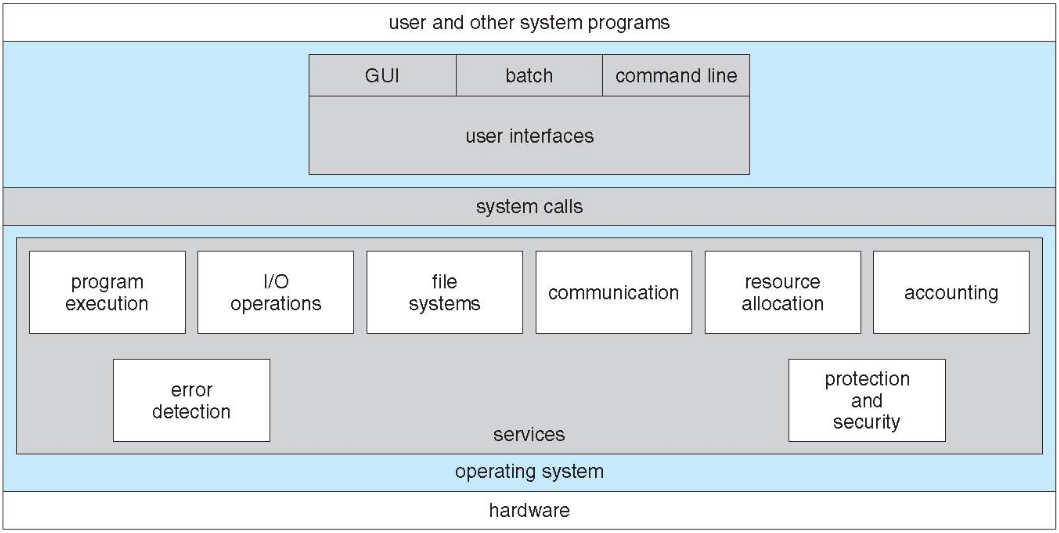
\includegraphics[width=\textwidth]{Pictures/InterfacciaUtente.png}
\caption{Stack del sistema operativo}
\end{figure}
\section{System call}
Le system calls forniscono l'interfaccia tra i processi e i servizi offerti dal sistema operativo. Sono tipicamente scritte in linguaggio di alto livello come C o C++, qualcuna in assembler, 
\subsection{Implementazione}
Tipicamente un numero viene associato ad ogni system call e l'interfaccia delle chiamate di sistema mantiene una tabella indicizzata secondo essi. L'interfaccia invoca la system call usata nel kernel del sistema 
operativo e poi ritorna lo stato della system call e gli eventuali valori di ritorno. Il chiamante non ha necessit\`a di conoscere come la system call \`e implementata. Mascherano pertanto i dettagli implementativi 
del sistema operativo fornendo un livello di astrazione intermedio. Sono chiamate da programmi attraverso l'interfaccia per la programmazione di applicazioni (Application Program Interface - API) di alto livello
piuttosto che usate direttamente. 
\subsubsection{API}
Le due APIs pi\`u comuni sono Win32 API per Windows e POSIX API per sistemi POSIX (portable operating-system interface for Unix) e le Java API per la Java virtual machine. Le API dovrebbero garantire la 
portabilit\`a delle applicazioni almeno sullo stesso tipo di API. 